\documentclass{scrartcl}

\usepackage{graphicx}
\usepackage{tikz}
\usepackage{caption}

\begin{document}
\begin{figure}
	\begin{minipage}[b]{0.5\textwidth}
	\centering
		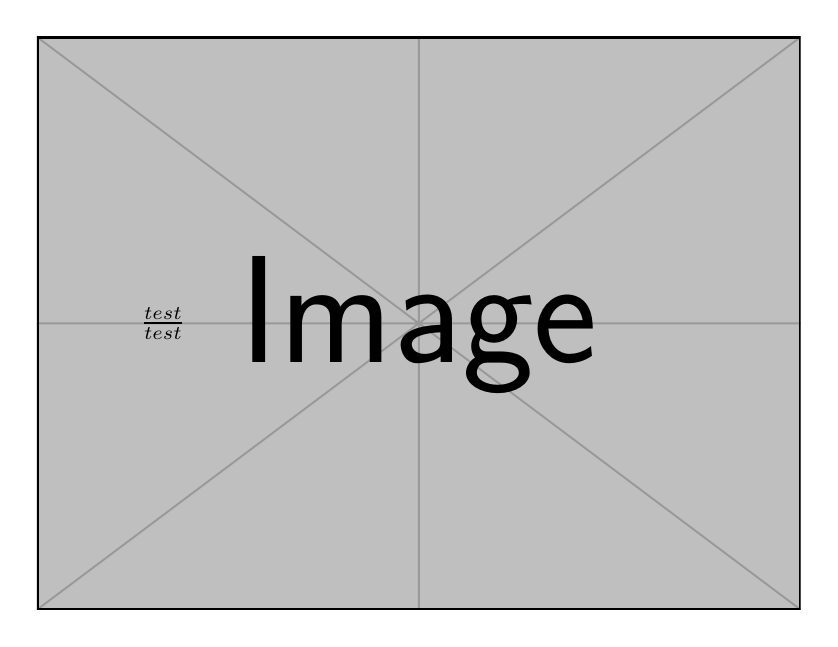
\begin{tikzpicture}
			\node (image) at (0,0) {\includegraphics[width=0.8\textwidth]{example-image}};
			\node (ylabel) at (-3.25,0) {$\frac{test}{test}$};
		\end{tikzpicture}
		\captionsetup{type=figure,font=footnotesize,justification=centering,margin={1cm,0.4cm},format=plain}
		\captionof{figure}{This is some junk text as caption for figure 1}
		\noindent\rule{1pt}{6pt}
		\noindent\rule{\textwidth}{1pt}
	\end{minipage}
	\begin{minipage}[b]{0.5\textwidth}
	\centering
		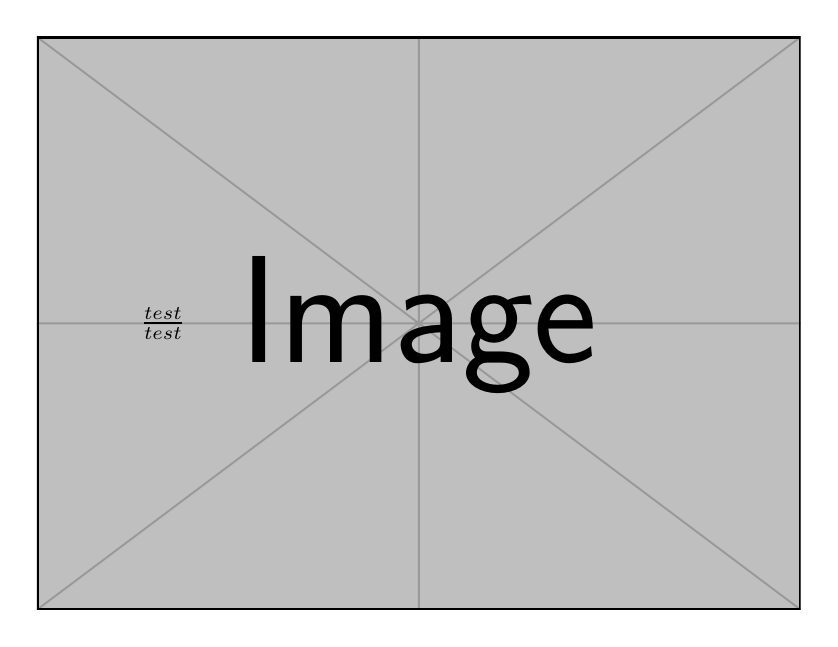
\begin{tikzpicture}
			\node (image) at (0,0) {\includegraphics[width=0.8\textwidth]{example-image}};
			\node (ylabel) at (-3.25,0) {$\frac{test}{test}$};
		\end{tikzpicture}
		\captionsetup{type=figure,font=footnotesize,justification=centering,margin={1cm,0.4cm},format=plain}
		\captionof{figure}{This is some junk text as caption for figure 2}
		\noindent\rule{1pt}{6pt}
		\noindent\rule{\textwidth}{1pt}

	\end{minipage}
\end{figure}
\end{document}